\documentclass[11pt,a4paper]{article}
\usepackage[margin=1in]{geometry}
\usepackage[T1]{fontenc}
\usepackage{lmodern,microtype,amsmath,amssymb,booktabs,tabularx,array,enumitem,graphicx,tikz}
\usepackage[hidelinks]{hyperref}
\usepackage{xcolor}
\definecolor{passgreen}{HTML}{25684D}
\definecolor{failred}{HTML}{A74429}
\definecolor{unknownamber}{HTML}{946D1F}
\newcommand{\okzero}{\textcolor{passgreen}{0}}
\newcommand{\badcount}[1]{\textcolor{failred}{\textbf{#1}}}
\newcommand{\unknowncount}[1]{\textcolor{unknownamber}{\textbf{#1}}}
\setcounter{topnumber}{3}
\setcounter{totalnumber}{5}
\renewcommand{\topfraction}{0.94}
\renewcommand{\textfraction}{0.06}
\renewcommand{\floatpagefraction}{0.7}
\usetikzlibrary{positioning,arrows.meta}
\setlength{\parindent}{0pt}
\setlength{\parskip}{5pt}
\setlength{\emergencystretch}{3em}
\renewenvironment{abstract}{\begin{center}\bfseries Abstract\end{center}}{}
\setlist{nosep,leftmargin=*}
\newcommand{\code}[1]{\nolinkurl{#1}}
\newcommand{\term}[1]{\textbf{#1}}
\title{Pathway: Natural-Language Course Planning with\protect\\Explicit Constraints and Timetable Verification}
\author{CS3263 Group 1}
\date{9 November 2026}
\begin{document}
\hypersetup{pageanchor=false}
\begin{titlepage}
\centering
\vspace*{1.5cm}
{\Large CS3263 Foundations of Artificial Intelligence\par}
\vspace{1.2cm}
{\huge\bfseries Pathway\par}
\vspace{0.4cm}
{\Large Natural-Language Course Planning with\\Explicit Constraints and Timetable Verification\par}
\vspace{1.8cm}
\begin{tabular}{lll}
\toprule
Name & Matriculation number & Email\\
\midrule
Sun Jiaen & A0288438L & E1309958@u.nus.edu\\
Shen Jingtao & A0287914N & E1297756@u.nus.edu\\
Achar Pavithra & A0305963Y & E1375774@u.nus.edu\\
\bottomrule
\end{tabular}
\vfill
{\large Project report\par}
9 November 2026
\vspace{1cm}
\begin{minipage}{0.9\textwidth}
\textbf{Scope of this version.} The report describes the current implementation and the archived exploratory experiments. Human ratings have not yet been collected. It makes no claim that the system certifies complete NUS graduation eligibility. The title page and references are separate from the numbered report body.
\end{minipage}
\end{titlepage}
\hypersetup{pageanchor=true}
\setcounter{page}{1}

\begin{abstract}
We present Pathway, a course planner that translates natural-language goals into editable constraint cards and uses constraint optimisation to construct a degree plan. The system combines semester assignment with whole-class weekly timetable search, independent academic checks and NUSMods export. Its reference snapshot contains 338 real courses and templates for Mathematics and Quantitative Finance minors. We evaluate direct LLM-generated plans against the necessary requirements implemented in the CSP, including prerequisite order, foundation coverage, minimum units and curriculum groups. A separate analysis checks semester offerings, exams and weekly feasibility. The archived experiment covers 15 model IDs under three rule-disclosure conditions. Only evaluable schedules receive compliance scores; unavailable or truncated responses remain unscored. We also prepare 15 anonymous schedules for two internal raters, with explicitly pending qualitative results. The system makes its checks inspectable, but bounded search and incomplete curriculum coverage limit its guarantees.
\end{abstract}

\section{Introduction}
A useful course plan must satisfy academic rules rather than merely list plausible courses. Prerequisites must precede dependent courses, curriculum groups require suitable selections, and courses placed together must admit a compatible weekly timetable. Students also have personal goals, such as finishing in eight semesters or completing a minor. These requirements interact across a multi-year plan.

Our question is whether direct language-model planning satisfies the same explicit rules as a symbolic planner. Students inspect the interpreted rules, a CSP searches assignments, and an independent checker tests the result. Contributions include the web application, integrated degree/weekly search, real-course/minor data and an auditable evaluation.

\section{Background and task}
Christou et al.~\cite{christou} model personalised course planning using mixed integer programming. NL4Opt~\cite{nl4opt} studies translation through an intermediate optimisation representation. The LLM-Modulo perspective~\cite{modulo} motivates external verification, while NavGPT~\cite{navgpt} illustrates explicit separation between model decisions and execution in navigation. Pathway applies these ideas to a restricted curriculum schema and adds feedback between semester and weekly search; it does not implement the full bidirectional LLM-Modulo framework.

\begin{figure}[htbp]
\centering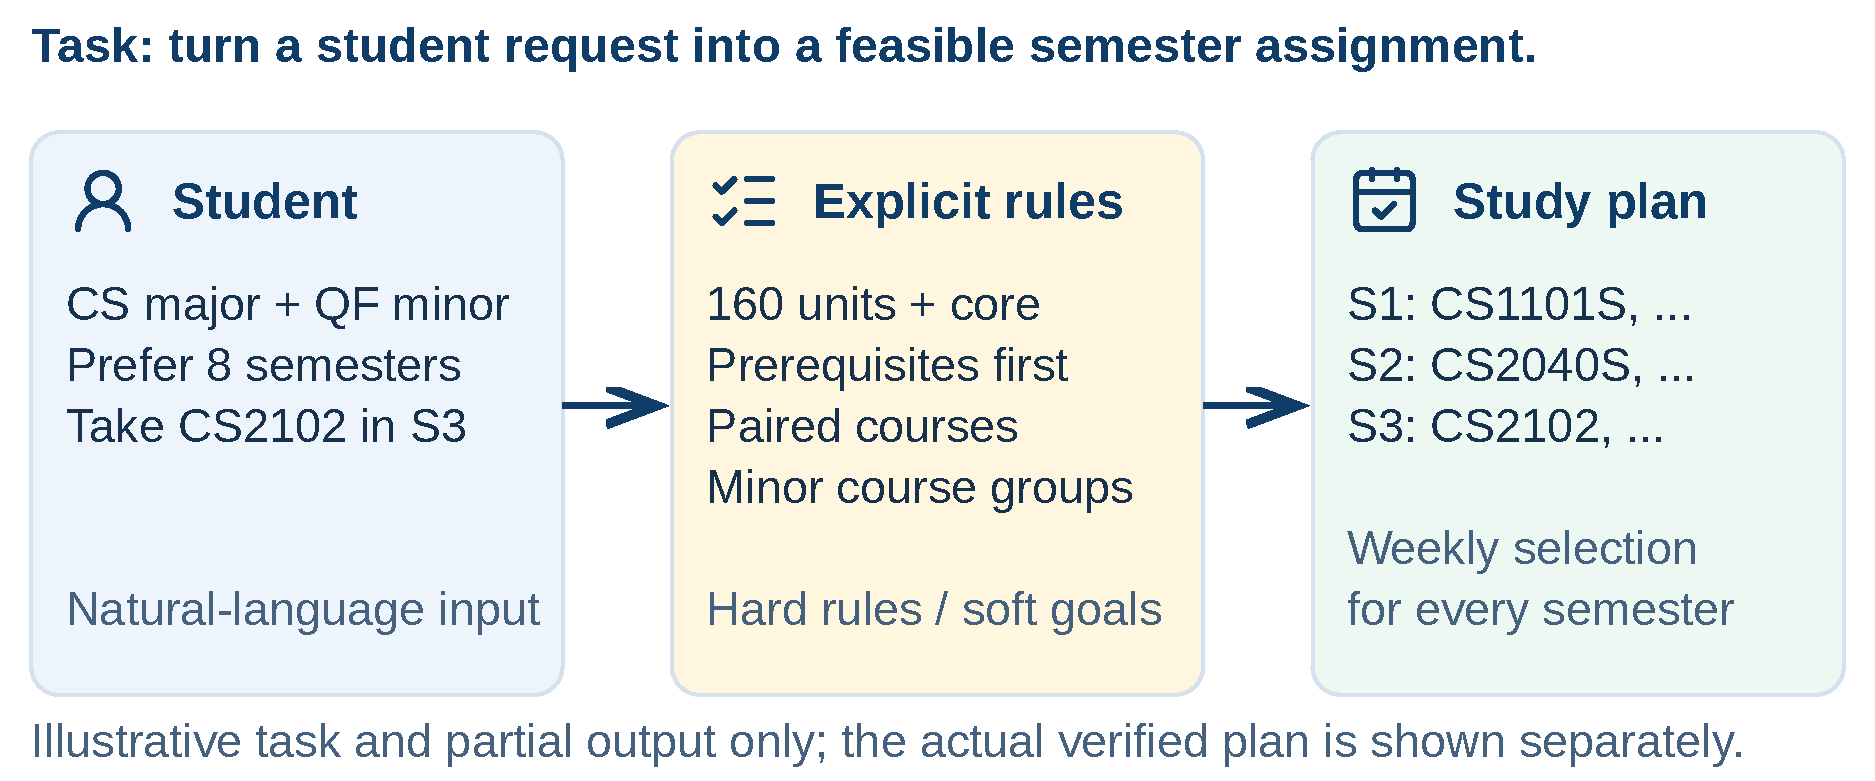
\includegraphics[width=\textwidth]{figures/task.pdf}
\caption{Task specification. A student's degree/minor commitments and preferences become explicit rules and a semester assignment. The example output is illustrative and incomplete.}\label{fig:task}
\end{figure}

Figure~\ref{fig:task} distinguishes \emph{requirements}, which must hold, from \emph{preferences}, which guide optimisation. Experiments assume a new AY2026/27 CS student, no completed university courses, H2 Mathematics and English entry eligibility, and a ten-semester horizon. Future years reuse AY2026/27 offerings, examinations and weekly patterns as a project assumption. Entry exemptions do not count university courses as completed.

\section{Method}
\subsection{Data and constraint inventory}
NUSMods supplies units, prerequisite trees, offerings, exams and lesson packages~\cite{nusmods}. Official CS, common curriculum and GE sources supply degree-related lists~\cite{nuscs,nuscommon,nusge}; official programme tables supply the minor templates~\cite{mathminor,qfminor}. The frozen catalogue contains 281 original and 57 supplementary courses. Of 338 entries, 272 pass the prototype's automatic eligibility filter, and 218 contain prerequisite trees. Graduate-level courses and year-long GEN variants are browse-only. Supplementary courses enter the active pool through a minor or explicit request and prerequisite closure.

Membership lists contain 23 ID, 17 CD, 4 GEA, 35 GEC, 28 GESS and 27 GEN courses. Membership can overlap; these counts are not counts of independent constraints. Placeholder labels such as ID1 or GEC never become course assignments. Distinct allocation variables assign real courses to curriculum buckets.

\begin{table}[htbp]\centering
\begin{tabularx}{\textwidth}{@{}lclX@{}}\toprule
Category & Cards & Strength & Implemented checks\\\midrule
Degree & 2 & Hard & At least 160 units and all 15 foundation courses.\\
Academic order & 2 & Hard & Earlier prerequisite trees; CS2101/CS2103T pairing.\\
Offering/time & 3 & Hard & Offered semester, exam compatibility, weekly selection.\\
Workload & 1 & Hard & 16--24 units per active semester; initially at most 20.\\
Focus & 1 & Hard & Three AI primary courses, including a level-4000+ course.\\
Common curriculum & 5 & Hard & Four units per GEC/GEA/GESS/GEN bucket; 12 distinct ID/CD units, at least two ID courses and at most one CD-only course.\\
Personal goals & 2 & Soft & Prefer finishing by semester 8 and 20-unit active semesters.\\\bottomrule
\end{tabularx}
\caption{Sixteen default cards: 14 hard and two soft. Workload bounds and the selected AI focus are editable project settings. Official sources are linked on applicable product cards.}\label{tab:inventory}
\end{table}

The schema supports 16 rule types: minimum units, required/excluded courses, prerequisites, corequisites, availability, exams, weekly feasibility, category units, course-in-semester, finish-by, semester bounds, workload target, blocked semesters, focus and minor programme. One user card may contain several rules of the same strength. Only course-in-semester, finish-by and workload-target rules support soft penalties.

The foundation set is CS1101S, CS1231S, CS2030S, CS2040S, CS2100, CS2101, CS2103T, CS2106, CS2109S, CS3230, ES2660, IS1108, MA1521, MA1522 and ST2334. A plan containing 160 units can still fail this mandatory-course check.

The Mathematics template requires 20+ units: eight foundation units, two intermediate courses worth at least eight units and an advanced course worth at least four units. QF requires QF1100, QF2104, QF3101, a four-unit mathematics option and an approved advanced elective. Both use distinct group allocations, at least 12 distinct units and at most eight shared units, subject to the implemented sharing policy~\cite{minorsharing}. A course counts once in the degree total and at most twice across programme uses. Explicit supplementary-course preclusions are checked. Full exemptions, grade/programme eligibility and EduRec declaration remain manual.

\subsection{Architecture and language interpretation}
\begin{figure}[htbp]
\centering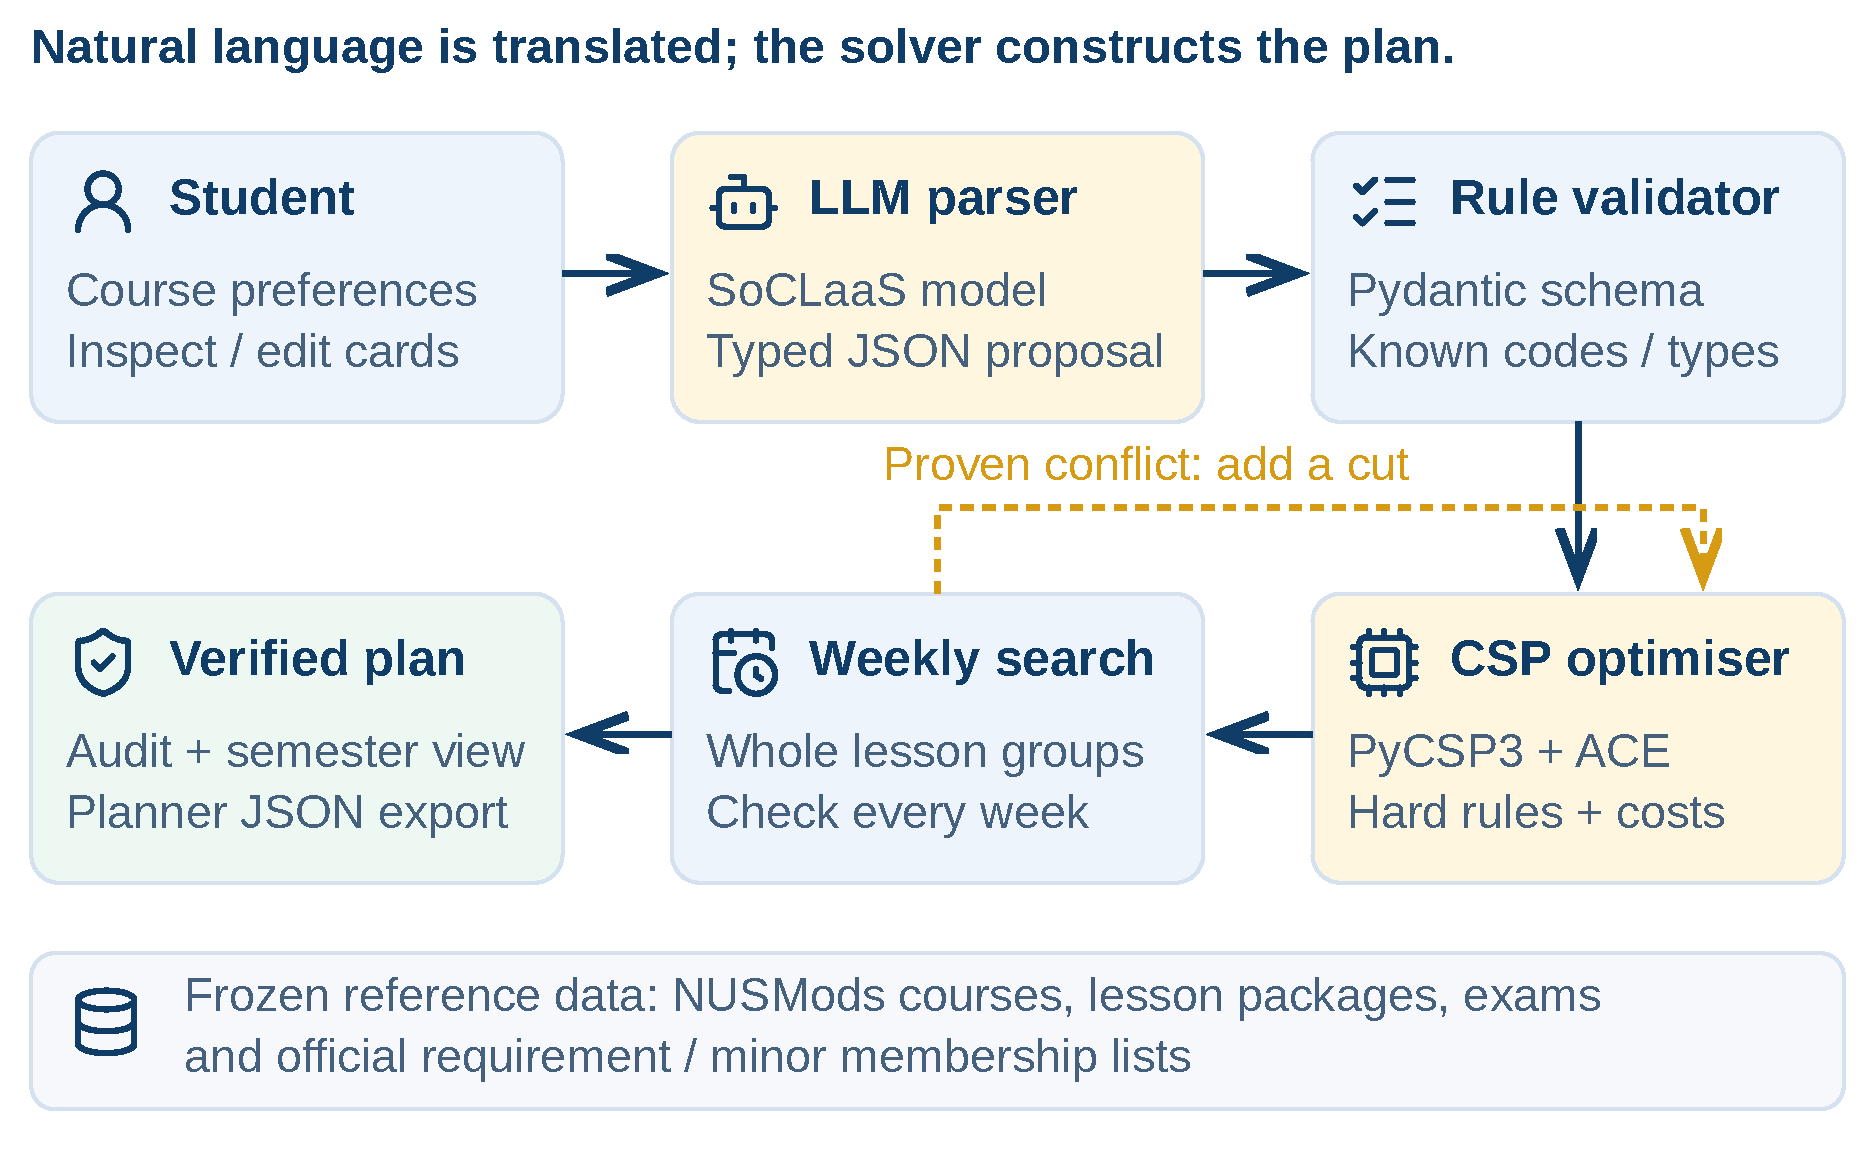
\includegraphics[width=\textwidth]{figures/architecture.pdf}
\caption{Architecture with explicit roles. The student inspects cards, the LLM proposes typed JSON, and the CSP constructs a plan. Proven weekly conflicts return as cuts to the optimiser. The frozen data supports interpretation, compilation and checking. Icons: Lucide, ISC licence.}\label{fig:architecture}
\end{figure}

The buildless frontend calls FastAPI. The server supplies SoCLaaS with the instruction, current cards, catalogue and allow-listed schema. Pydantic rejects unknown courses/types, unsupported hard/soft combinations and out-of-horizon semesters. Unsupported or ambiguous requests should produce clarification without new cards. Schema validity does not prove semantic fidelity; students can inspect, edit or remove cards before searching. Deleting a card removes its active rules; reset restores the defaults.

The compiler uses bundled PyCSP3 2.6.1 and Java ACE-2.6~\cite{pycsp,ace}. Each solve runs in an isolated process whose environment omits SoCLaaS credentials. Figure~\ref{fig:architecture} shows the separation between language, constraint compilation and verification.

\subsection{CSP formulation and preferences}
For course $c$, $x_c\in\{0,\ldots,H\}$ denotes omission or its semester. With units $u_c$, semester load and degree units are
\[
L_s=\sum_c u_c[x_c=s],\qquad U=\sum_c u_c[x_c>0].
\]
Hard cards constrain these variables and group allocations. A selected course requires its AND/OR/at-least-$n$/supported-cohort prerequisite tree to hold, with every required course $p$ strictly earlier: $0<x_p<x_c$. Unknown tree formats fail closed. Corequisite pairing is $x_{\rm CS2101}=x_{\rm CS2103T}$.

For soft pin rules $P$, finish targets $F$ and workload targets $W$, the objective is
\[
U+10^5\!\sum_{(c,s)\in P}[x_c\ne s]
+10^4\!\sum_{t\in F}\sum_c[x_c>t]
+100\!\sum_{w\in W}\sum_s[L_s>0]|L_s-w|.
\]
This is a weighted sum, not a proved lexicographic order. Hard violations cannot be offset by preference rewards. The units term discourages gratuitous courses; a bounded feasible result need not be optimal.

\subsection{Weekly refinement and independent checks}
Weekly search chooses one complete class package per lesson type, retaining all its meetings. A clash requires overlapping days, time intervals and teaching weeks. Exams are checked separately. CS2101 shares the matching CS2103T package and must accompany it: this is a user-confirmed project mapping for missing separate CS2101 times. Integrated AY2026/27 groups are retained whole, without guessing which meetings to remove.

\begin{quote}
\textbf{Algorithm 1: degree/weekly refinement}\par
1. Compile active hard rules, allocation variables, weighted preferences and cheap fixed-class conflict cuts.\par
2. Run ACE for up to four seconds; retain a feasible incumbent if available.\par
3. Check every active semester using whole-class search, bounded at 100,000 nodes. Missing data or timeout remains unknown.\par
4. For a proven incompatible set $K$, shrink it and add $\sum_{c\in K}[x_c=s]<|K|$ for each semester of matching reference parity; solve again.\par
5. Stop after at most 12 attempts, the approximate 80-second refinement budget or the 110-second outer timeout. Recheck before returning a verified plan.
\end{quote}

The independent ordinary-Python validator rechecks hard rules and allocations. It shares data and some helper semantics with the compiler, so common modelling errors remain possible. Foundation coverage and prerequisite order are always audited: deleting those cards can produce an exploratory preview, but an academically invalid preview cannot be exported. Experiments disallow conditional plans with unpublished lessons.

\subsection{Implemented product}
\begin{figure}[htbp]
\centering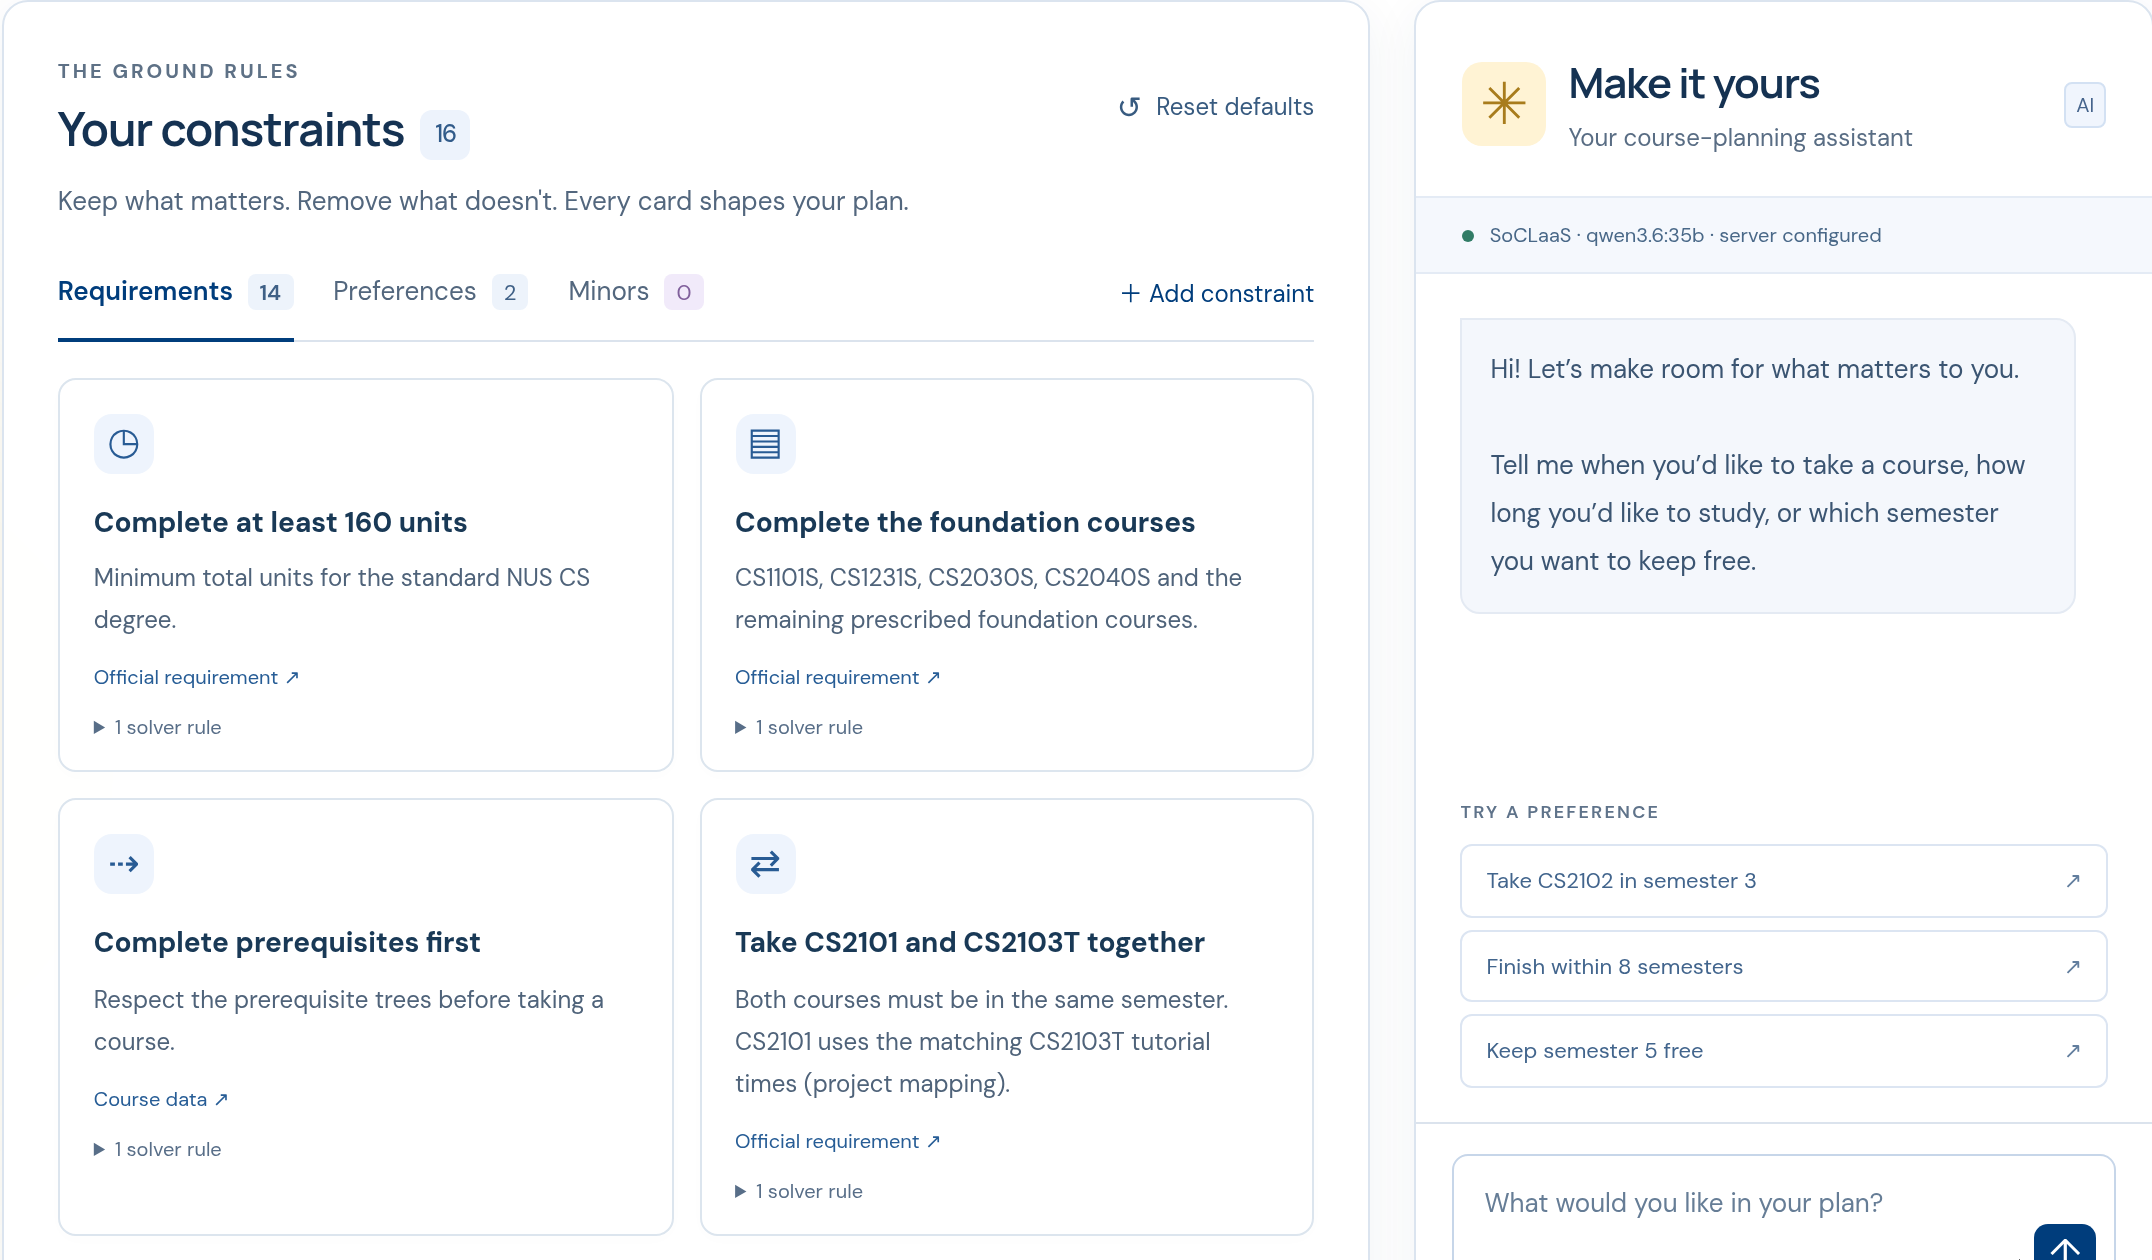
\includegraphics[width=\textwidth]{figures/planner_workspace.png}
\caption{Actual Pathway requirement editor and planning assistant, cropped to the first requirement cards. Requirements, preferences and minors are separate tabs; applicable cards link to their sources.}\label{fig:product}
\end{figure}

\begin{figure}[htbp]
\centering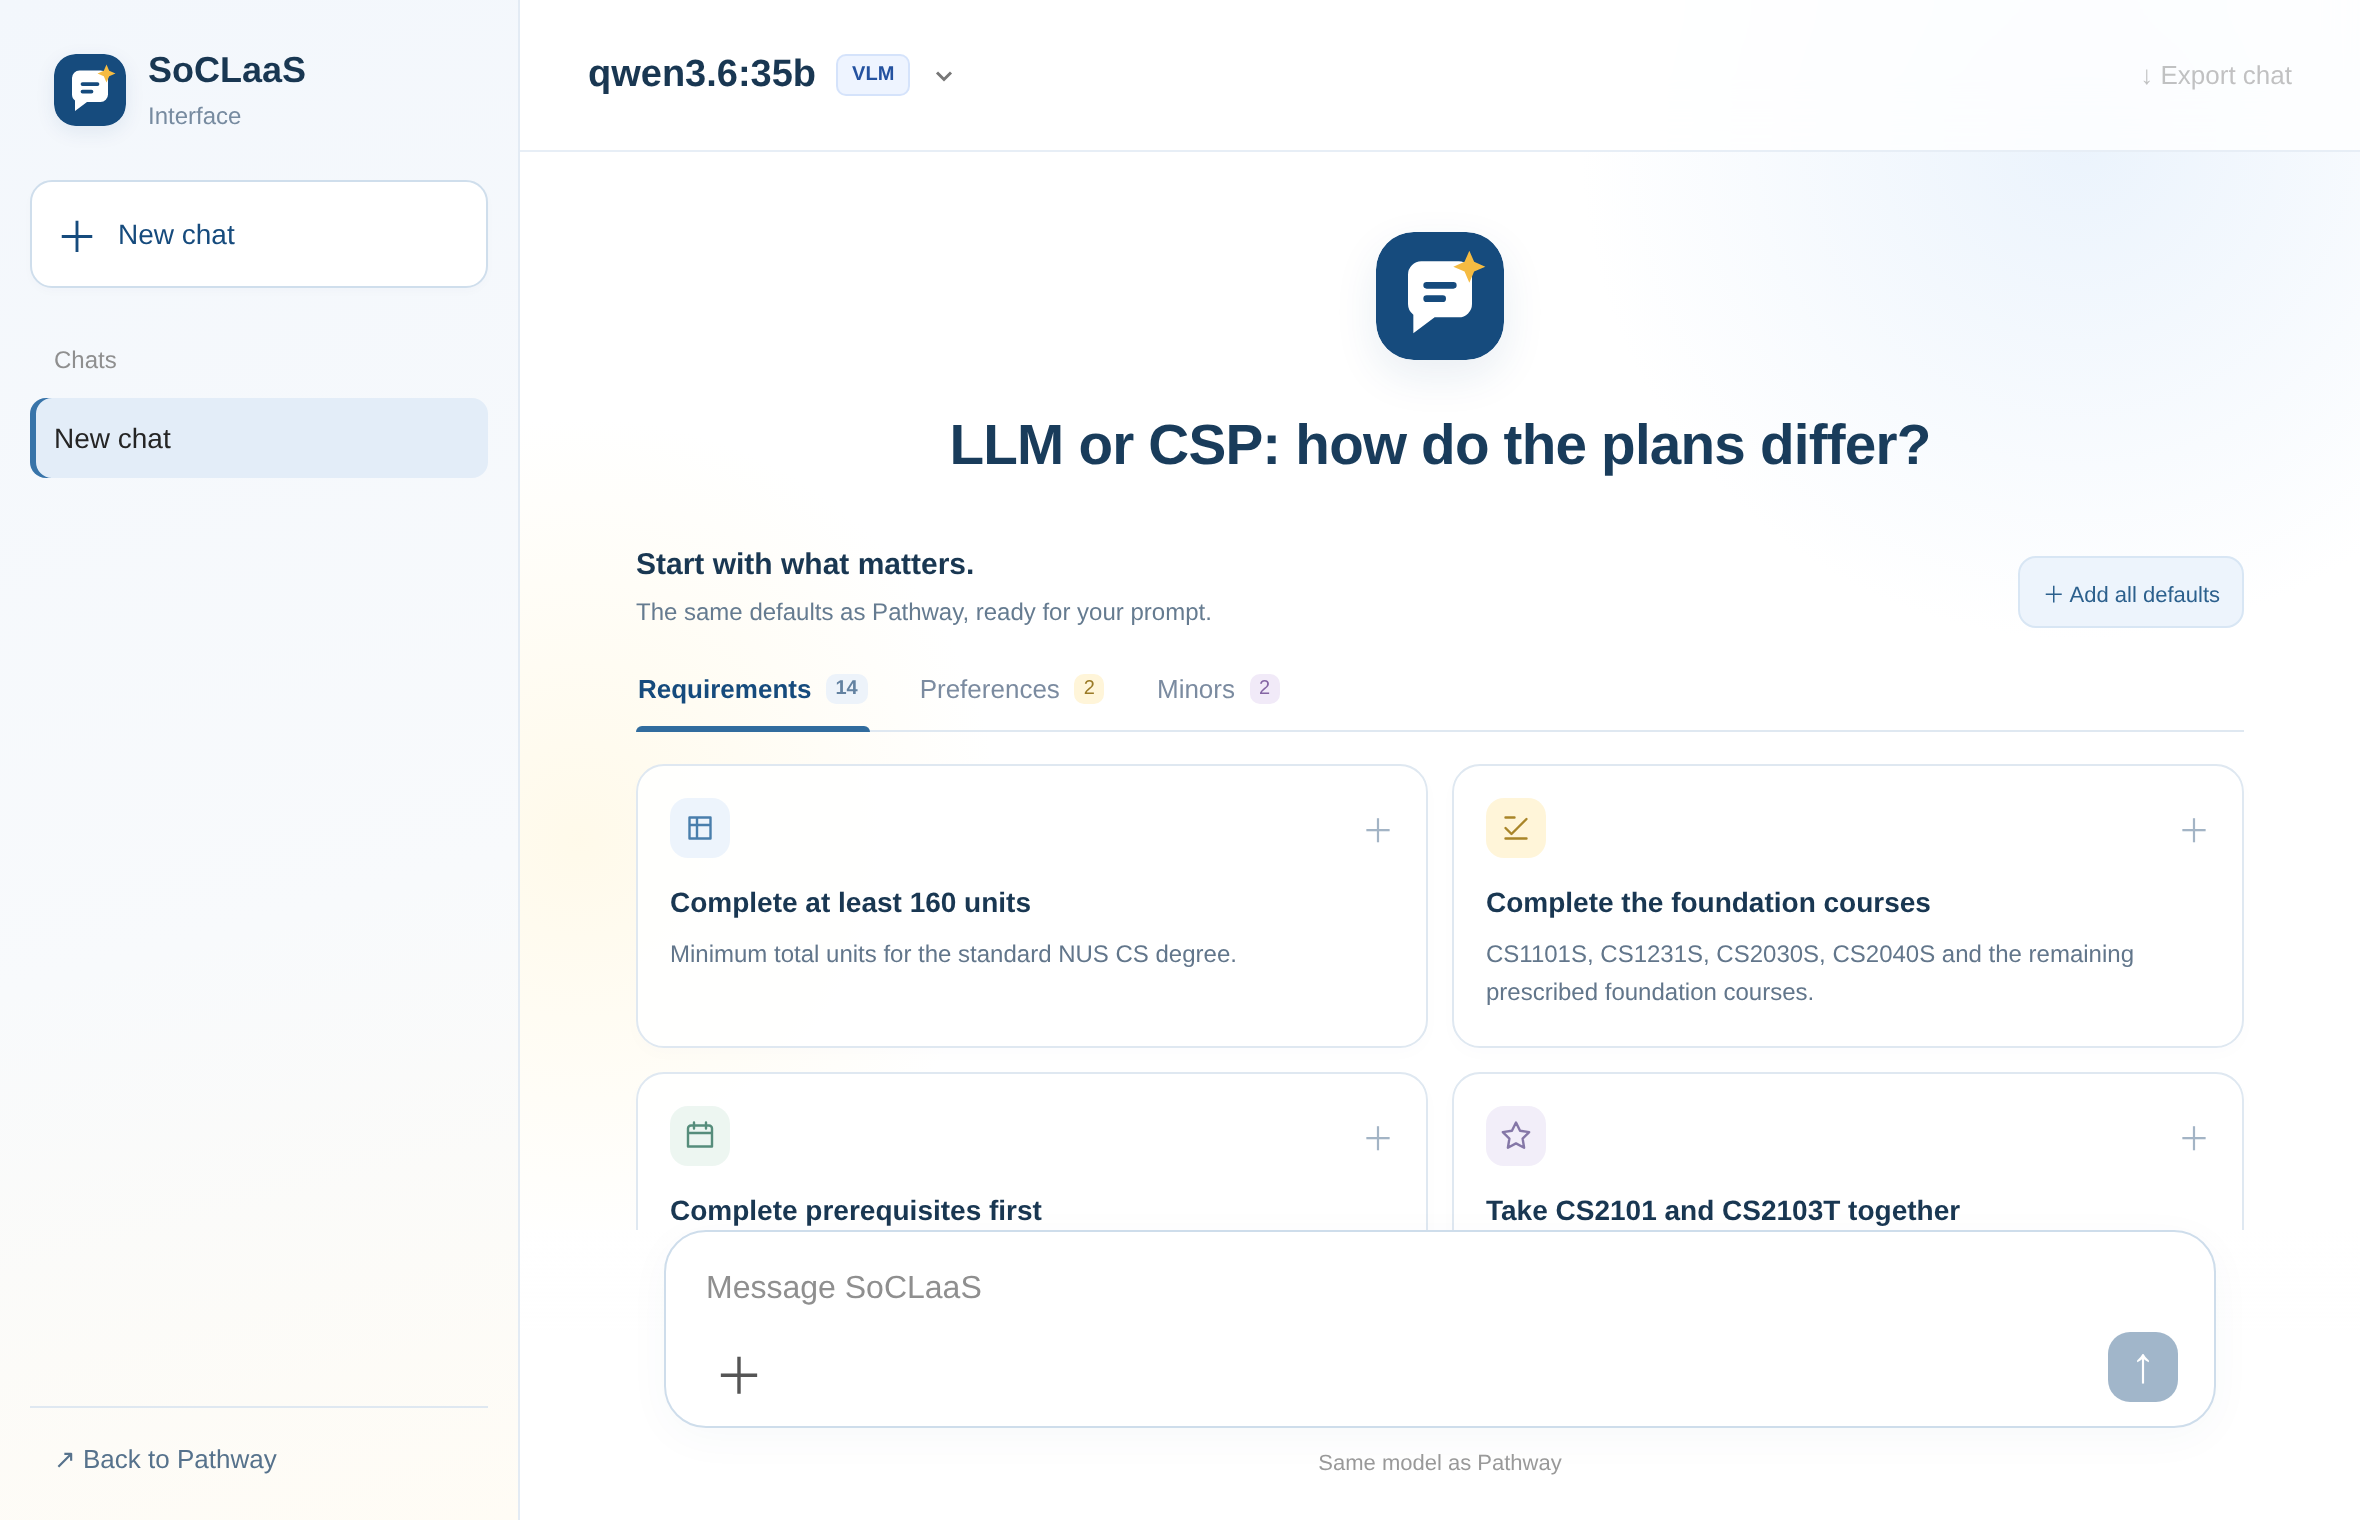
\includegraphics[width=\textwidth]{figures/soclaas_interface.png}
\caption{Actual SoCLaaS Interface used for direct-model interaction. Its requirement, preference and minor prompts mirror Pathway. The model selector changes the requested model; no solver is invoked by direct chat.}\label{fig:direct-ui}
\end{figure}

\begin{figure}[htbp]
\centering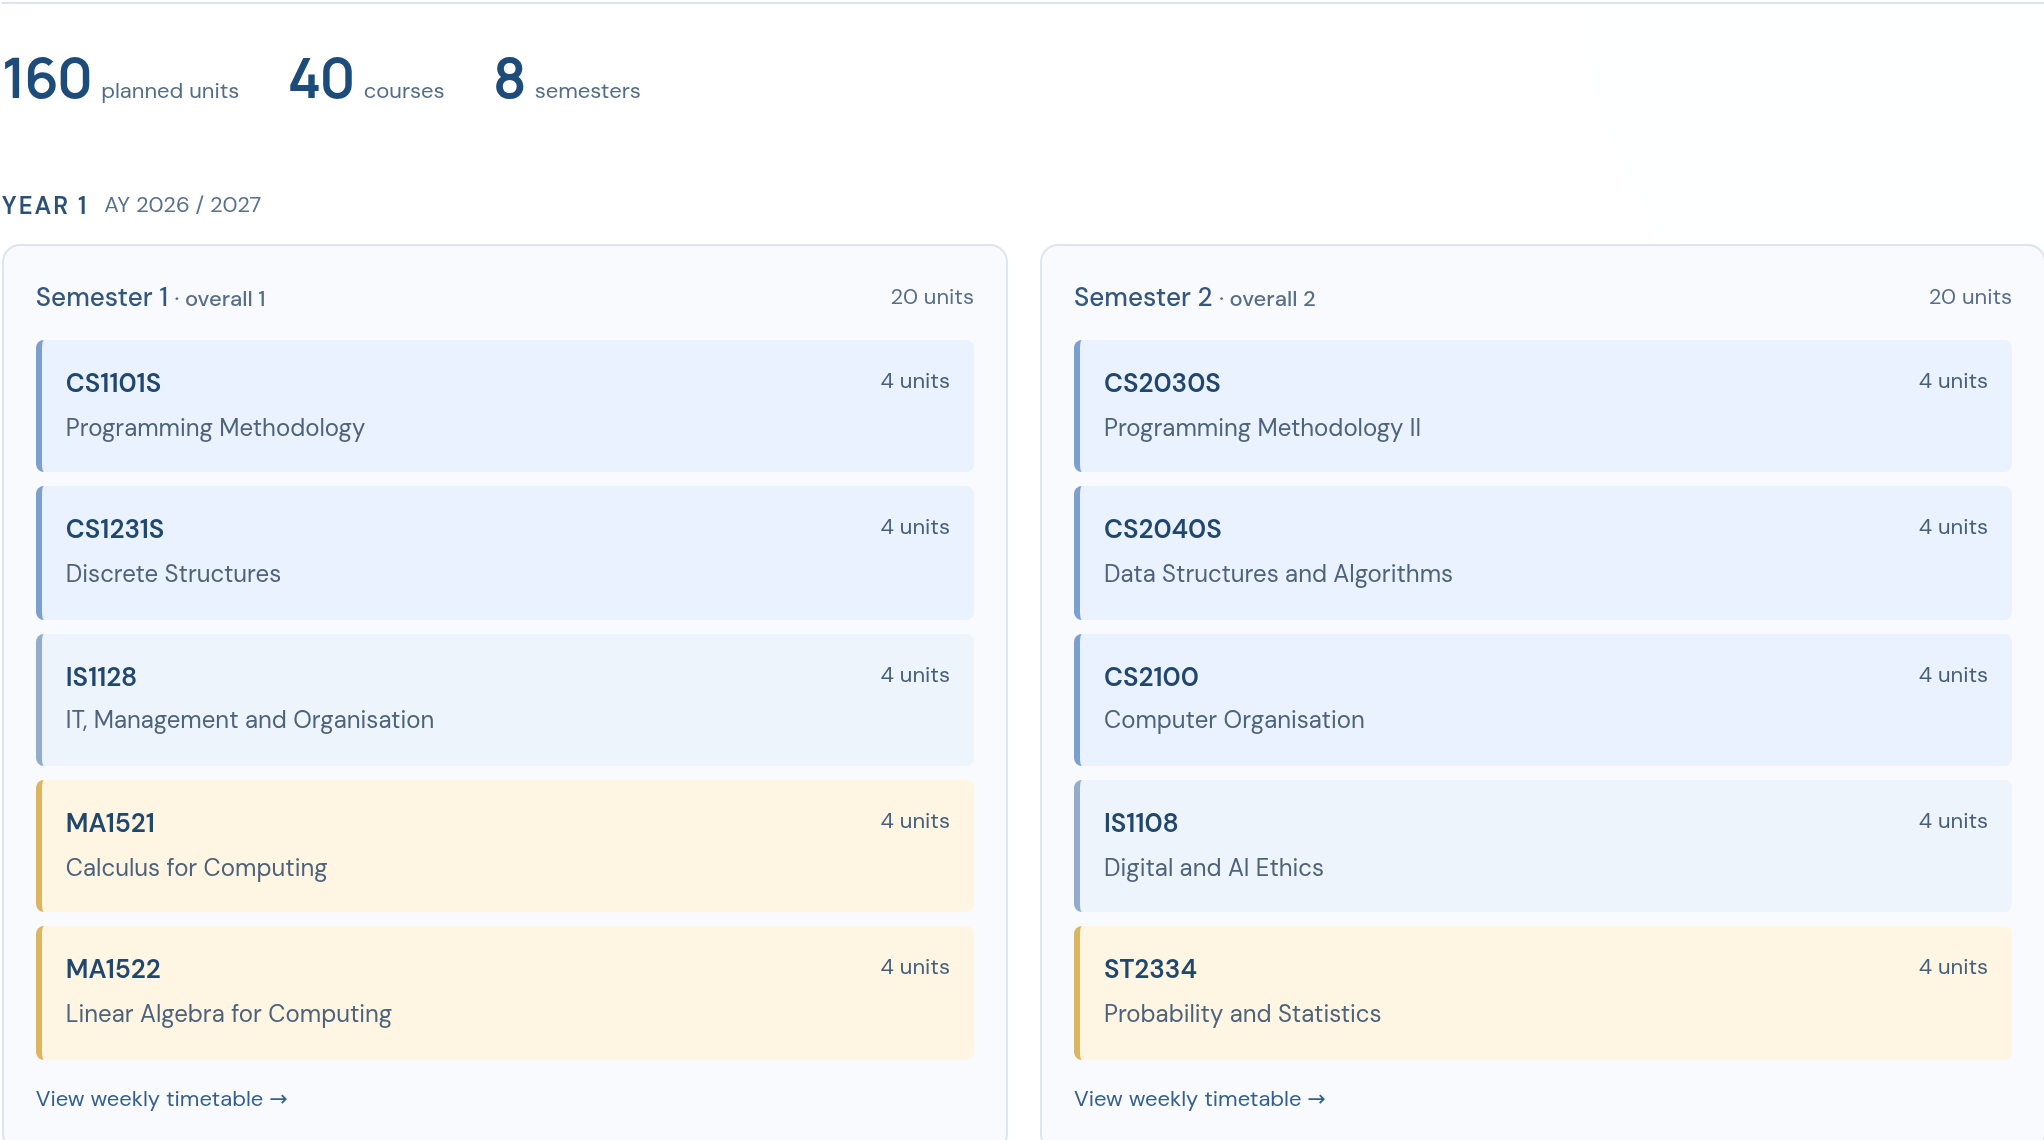
\includegraphics[width=\textwidth]{figures/degree_plan.png}
\caption{Actual semester-plan view displaying the archived verified base run: 160 units, 40 courses and eight semesters. The crop shows Year 1. Every semester links to a weekly view, and the product exports native NUSMods Planner JSON. Screenshots use an isolated browser profile; this saved solver response is replayed without inventing courses or outcomes.}\label{fig:degree}
\end{figure}

Full-resolution screenshots, the weekly view, editable diagrams and capture provenance accompany the source package.

\section{Experiments}
\subsection{Design and necessary-requirement metrics}
We test whether generated plans satisfy the necessary rules encoded in \code{backend/solver_adapter.py} and rechecked in \code{backend/validation.py}. All methods receive the same frozen NUSMods/course-group facts and a JSON semester-array output contract. The three conditions disclose \textbf{A}: assumptions; \textbf{AP}: assumptions plus preferences; \textbf{APR}: assumptions, preferences and hard requirements. Catalogue membership facts remain visible throughout, so this is a rule-instruction disclosure experiment.

Thirteen canonical SoCLaaS chat models plus the exact Astra and Sol IDs~\cite{openai} give 45 main calls: 15 models $\times$ three conditions, one response per cell. Aliases, embeddings and transcription models are excluded. SoCLaaS uses temperature 0, a 3,500-token cap and no system prompt, tools, repair or retry. Astra and Sol use Codex CLI, medium reasoning and an empty read-only directory with user rules/configuration disabled; tool-using runs are rejected. Hidden CLI instructions and different generation limits prevent a fully API-controlled comparison. The appendix preserves the exact model IDs, metadata, prompts, raw responses, source/data hashes and settings.

\textbf{Academic compliance is the primary outcome.} For each evaluable plan we count: selected courses whose prerequisite tree is unsatisfied; missing courses from the 15-course foundation set; unit shortfall $\max(0,160-U)$; failed AI-focus rule; failed GE/ID buckets; and a violated CS2101/CS2103T pairing. These diagnostics separate missing courses, unit deficits and requirement failures. GE/ID uses actual allocation and distinctness rules. Zeroes in these columns mean only that those implemented academic checks pass.

\textbf{Scheduling checks are separate.} We count assignments to unavailable reference semesters, overlapping exam pairs, semesters with proven weekly incompatibility, unverified weekly semesters and violations of the project workload bounds. An unknown check is not a proven conflict. The parser rejects empty/malformed schedules; unknown/duplicate/ineligible course codes are explicit structural failures. Bounded existential allocation search avoids requiring direct models to output private solver variables. Unresolved allocation prevents full verification.

\subsection{Quantitative results: do generated plans meet the requirements?}
\begin{table}[htbp]\centering
\begin{tabular}{@{}llrrrrrr@{}}\toprule
Method & Input & Prereq. & Core & Units & Focus & GE/ID & Pair\\\midrule
Qwen 3.6 & A & \badcount{21} & \badcount{2} & \okzero & \okzero & \badcount{2} & \okzero \\
Qwen 3.6 & AP & \badcount{4} & \badcount{2} & \okzero & \badcount{1} & \badcount{2} & \okzero \\
Qwen 3.6 & APR & \badcount{5} & \okzero & \okzero & \okzero & \badcount{2} & \okzero \\
\addlinespace[2pt]
Qwen Coder & A & \badcount{8} & \badcount{2} & \okzero & \badcount{1} & \badcount{1} & \okzero \\
Qwen Coder & AP & \badcount{2} & \badcount{2} & \okzero & \badcount{1} & \badcount{1} & \okzero \\
Qwen Coder & APR & \okzero & \okzero & \okzero & \okzero & \badcount{1} & \okzero \\
\addlinespace[2pt]
Qwen VL & A & \badcount{7} & \badcount{2} & \okzero & \okzero & \badcount{4} & \okzero \\
Qwen VL & AP & \badcount{5} & \badcount{2} & \okzero & \badcount{1} & \badcount{5} & \okzero \\
\addlinespace[2pt]
Astra & A & \okzero & \okzero & \okzero & \badcount{1} & \okzero & \okzero \\
Astra & AP & \badcount{1} & \okzero & \okzero & \okzero & \okzero & \okzero \\
Astra & APR & \okzero & \okzero & \okzero & \okzero & \okzero & \okzero \\
\addlinespace[2pt]
Sol & A & \badcount{1} & \badcount{1} & \okzero & \okzero & \okzero & \okzero \\
Sol & AP & \okzero & \okzero & \okzero & \badcount{1} & \okzero & \okzero \\
Sol & APR & \okzero & \okzero & \okzero & \okzero & \okzero & \okzero \\
\addlinespace[2pt]
\midrule
Pathway CSP & APR & \okzero & \okzero & \okzero & \okzero & \okzero & \okzero \\
\bottomrule\end{tabular}
\caption{Violations of implemented academic requirements; lower is better. Prereq.: courses with an unsatisfied earlier-prerequisite tree. Core: missing foundation courses. Units: deficit below 160. Focus: failed AI-focus rule (0/1). GE/ID: failed GEC, GEA, GESS, GEN or ID/CD buckets (0--5). Pair: failed CS2101/CS2103T pairing (0/1). Every row is one actual generated plan; no error response is scored as a plan.}\label{tab:academic}
\end{table}

\begin{table}[htbp]\centering
\begin{tabular}{@{}lrrrrr@{}}\toprule
Method (APR) & Offering & Exams & Weekly & Unknown & Load\\\midrule
Qwen 3.6 & \badcount{11} & \badcount{1} & \badcount{1} & \unknowncount{5} & \badcount{1} \\
Qwen Coder & \badcount{5} & \okzero & \badcount{1} & \unknowncount{4} & \okzero \\
Astra & \okzero & \okzero & \okzero & \unknowncount{1} & \okzero \\
Sol & \okzero & \okzero & \okzero & \okzero & \okzero \\
Pathway CSP & \okzero & \okzero & \okzero & \okzero & \okzero \\
\bottomrule\end{tabular}
\caption{Schedule-level checks under full rule disclosure. Offering counts courses assigned to an unavailable semester; Exams counts overlapping pairs; Weekly counts semesters with proven lesson incompatibility; Unknown counts semesters with missing lesson data or timeout; Load counts semesters outside the editable project workload bounds. Unknown is not a proven violation.}\label{tab:temporal}
\end{table}


Table~\ref{tab:academic} scores the 14 actual evaluable base schedules, preserving their input condition. Across all 45 requests, 12 had service/transport failures and 19 received unparseable, output-limited responses. These 31 calls are \emph{unscored}, not zero-violation schedules; complete coverage remains in the appendix. Thus the available compliance comparison contains five direct model IDs, not 15 successfully assessed models.

Under APR, Qwen 3.6 violates five course prerequisite trees and two GE/ID buckets. For example, it places CS1231S and CS2040S together in semester 2 without an earlier alternative satisfying the discrete-mathematics prerequisite. Same-semester enrolment cannot satisfy an earlier prerequisite. Qwen Coder passes prerequisite/foundation/unit/focus/pair checks but misses an ID/CD bucket. Astra and Sol pass all academic columns. Table~\ref{tab:temporal} reveals an additional distinction: Astra has an unverified weekly semester, whereas Sol passes every implemented hard check. Passing the graduation-related columns alone therefore does not establish a usable timetable. All 14 plans reach at least 160 units: unit quantity by itself does not ensure academic validity.

The base CSP control passes both tables and both default preferences. Minor controls also pass their active hard checks: Mathematics yields 177 units over nine semesters, missing duration and balance preferences; QF yields 162 units over eight semesters, missing balance. They are three typed-card controls, not 45 end-to-end parser trials. Two separately archived production-parser probes correctly represent the requested minor and soft CS2102 pin and subsequently solve; this is only a smoke test. Direct Sol also produces a fully verified plan, so the data do not establish an exclusive correctness advantage for CSP.

\subsection{Qualitative evaluation: design and pending results}
The packet contains 15 anonymous schedules: five methods on the base, Mathematics-minor and QF-minor tasks. Methods are Pathway CSP, Qwen 3.6, Qwen Coder, Astra and Sol. The predefined availability rule substitutes Qwen Coder for Llama, whose requests returned no evaluable plans. Two teammates independently rate all schedules in different recorded random orders. Displays use identical formatting and omit method identity, generated prose, runtime and automatic verdicts. The method key remains separate.

Five dimensions use explicit 1--5 anchors: preference satisfaction, apparent feasibility/actionability, workload/progression, clarity/verifiability and overall usefulness. Broadly, 1 indicates unusable or largely unmet goals, 3 a useful starting point needing substantial revision, and 5 a strong plan meeting the assessed criterion with routine checks. The packet defines every score separately for every dimension. Raters may leave uncertain judgements blank with a reason and identify concrete course/semester issues.

\begin{table}[htbp]\centering
\begin{tabular}{@{}lrrrrrr@{}}\toprule
Method & $n$ & Pref. & Feasib. & Progress & Clarity & Overall\\\midrule
Pathway CSP & 0/6 & TBC & TBC & TBC & TBC & TBC \\
Qwen 3.6 & 0/6 & TBC & TBC & TBC & TBC & TBC \\
Qwen Coder & 0/6 & TBC & TBC & TBC & TBC & TBC \\
Astra & 0/6 & TBC & TBC & TBC & TBC & TBC \\
Sol & 0/6 & TBC & TBC & TBC & TBC & TBC \\
\bottomrule\end{tabular}
\caption{Qualitative results template, not measured outcomes. TBC means to be collected; no numerical placeholder is a participant score. Each method has three tasks and two independent raters, giving six planned ratings per dimension. Final cells will report median [minimum, maximum] on the anchored 1--5 scale.}\label{tab:qualitative}
\end{table}


Table~\ref{tab:qualitative} is a visible reporting template with \textbf{no collected scores}. After collection, report per-rater scores, medians/ranges and within-task paired differences against CSP, retaining ties and missingness. Do not treat 30 plan-rater records as independent participants. Both raters are developers, so convenience sampling, recognition and expectation bias limit generalisation. No qualitative superiority claim is currently supported.

\section{Responsible AI}
Cards, source links, unmet-preference messages and audit diagnostics expose which rules were checked. This supports constraint-level interpretation, not an explanation of the LLM's internals or a guarantee of faithful translation. Human inspection remains necessary.

Credentials stay on the backend and are stripped from the solver worker. Model output is data, never executable code. Real messages can nevertheless reveal personal information to an external provider, and browser conversations persist locally. The experiments use synthetic profiles; no differential privacy or formal security audit is claimed. Allow-listed schemas restrict executable prompt-injection effects but cannot prevent an unwanted schema-valid rule.

Default AI focus and workload settings may poorly fit other interests, disabilities, employment or caring commitments. Keep these settings editable and avoid treating a longer degree as failure. Completion/units penalties omit course difficulty and can encourage demanding combinations. Adviser review and registration checks remain necessary; the product must not present itself as official graduation certification.

\section{Limitations and conclusion}
The schema and two curated minors cannot express arbitrary programmes such as a Mathematics second major. Full preclusions, exemptions, grade/programme restrictions, internships, SEP/NOC and CourseReg quotas are not modelled. Future offerings can change, invalidating the repeated-year assumption. Bounded search can fail without proving infeasibility, and weighted preferences need not yield the student's ideal plan.

The study has one base task, one response per disclosure cell and substantial output-budget/availability attrition. Frontier harness settings differ from SoCLaaS; the checker shares snapshot data and helper semantics with the compiler. Broader profiles, output-budget sensitivity, parser-fidelity testing and external curriculum review are needed before strong comparative claims.

Pathway demonstrates an implemented connection from student language to inspectable rules, semester optimisation, weekly refinement and NUSMods export. Its practical benefit is explicit, scoped checking of plans. Completing the independent ratings and expanding curriculum coverage are the next steps.

\section*{Contributions and AI assistance}
\textbf{Sun Jiaen:} frontend/backend, model integration, report and quantitative experiments. \textbf{Shen Jingtao and Achar Pavithra:} joint responsibility for the CSP algorithm; no unconfirmed division of algorithm subtasks is claimed.

OpenAI Codex assisted with implementation/debugging, source inspection, benchmark scripting/execution, writing, figures, presentation planning and evaluation materials. Astra, Sol and SoCLaaS models also served as experimental subjects. Screenshots document the real product; qualitative placeholders are explicitly unmeasured. The named authors must review the draft, citations, code and claims before submission and retain responsibility for the final work.


\clearpage
\begin{thebibliography}{99}
\bibitem{christou} I. T. Christou, E. Vagianou and G. Vardoulias. Planning Courses for Student Success at the American College of Greece. 2022. \url{https://arxiv.org/abs/2207.02659}.
\bibitem{nl4opt} R. Ramamonjison et al. NL4Opt Competition: Formulating Optimization Problems Based on Their Natural Language Descriptions. \emph{PMLR}, 220:189--203, 2022 competition proceedings. \url{https://proceedings.mlr.press/v220/ramamonjison23a.html}.
\bibitem{modulo} S. Kambhampati et al. Position: LLMs Can't Plan, But Can Help Planning in LLM-Modulo Frameworks. \emph{ICML}, PMLR 235:22895--22907, 2024. \url{https://proceedings.mlr.press/v235/kambhampati24a.html}.
\bibitem{navgpt} G. Zhou, Y. Hong and Q. Wu. NavGPT: Explicit Reasoning in Vision-and-Language Navigation with Large Language Models. 2023. \url{https://arxiv.org/abs/2305.16986}.
\bibitem{pycsp} C. Lecoutre and N. Szczepanski. PyCSP3: Modeling Combinatorial Constrained Problems in Python. 2020, revised 2026. \url{https://arxiv.org/abs/2009.00326}.
\bibitem{ace} C. Lecoutre. ACE, a generic constraint solver. 2023, revised 2024. \url{https://arxiv.org/abs/2302.05405}.
\bibitem{nusmods} NUSMods. API v2 and Planner. Accessed 9 November 2026. \url{https://api.nusmods.com/v2/}; \url{https://nusmods.com/planner}.
\bibitem{nuscs} NUS Computing. Computer Science, Cohort AY2026/2027. Accessed 9 November 2026. \url{https://www.comp.nus.edu.sg/cug/per-cohort/cs/cs-26-27/}.
\bibitem{nuscommon} NUS Computing. Common Curriculum requirements. Source URL retained in the frozen course snapshot. Accessed 9 November 2026. \url{https://www.comp.nus.edu.sg/cug/soc-22-23/}.
\bibitem{nusge} National University of Singapore. General Education. Source URL retained in the frozen course snapshot. Accessed 9 November 2026. \url{https://www.nus.edu.sg/registrar/academic-information-policies/undergraduate-students/general-education/list-of-courses-approved-under-the-ge-pillars}.
\bibitem{mathminor} NUS Department of Mathematics. Minor in Mathematics and AY2021/22-onwards requirements. Accessed 9 November 2026. \url{https://www.math.nus.edu.sg/ug/majmin/minors/mamin/}.
\bibitem{qfminor} NUS Department of Mathematics. Minor in Quantitative Finance and AY2021/22-onwards requirements. Accessed 9 November 2026. \url{https://www.math.nus.edu.sg/ug/majmin/minors/qfmin/}.
\bibitem{minorsharing} NUS Computing. Minor Programmes: double-counting policy. Accessed 9 November 2026. \url{https://www.comp.nus.edu.sg/programmes/ug/minorc/}.
\bibitem{openai} OpenAI. Model documentation: GPT-6 Astra and GPT-6.1 Sol. Accessed 9 November 2026. \url{https://developers.openai.com/api/docs/models}.
\end{thebibliography}
\end{document}
